\subsubsection*{T3.3 Solving the local control problem (..., TUD 2.5PM, ...)}

TUD hired a student for setting up the iCub hardware and simulation environment.
    

\subsubsection*{T3.4 Bootstrapping and validating the control approach in rigid world and compliant cases (..., TUD 8PM, INRIA 4PM)} 
    
During the second year, TUD continued their research in inverse dynamics model
learning in situations with contacts. A mixture of experts approach with
Gaussian processes was developed using tactile feedback from the iCub's sensor
skin. This approach was evaluated on the iCub robot, where the learned model
accurately predicts contact forces, is robust to changes in the environment and
outperforms existing analytic dynamic models that make use of force/torque
sensor data. 
An exemplary task is illustrated in Figure~\cite{fig:exp3:icuparis_experiment_bars} 
when obstacles are introduced on both sides of a planned circular motion.
In Figure~\cite{fig:exp3:gating} can be seen that the mixture-of-experts recognize the presence of the two different contacts and opportunely active the corresponding expert to compensate for the contact.
As a result, the torques predicted from our approach (red curve) closely follow the ground truth (blue curve) and outperform the analytic model (green curve).
A paper was published in an international robotics conference
\cite{Calandra_ICRA15}. A continuative study exploiting learned dynamics models
for control is in progress of writing. Both studies are detailed in Deliverable
D4.2.

	\begin{figure}[t]
		\begin{minipage}{.43\linewidth}
			\centering
			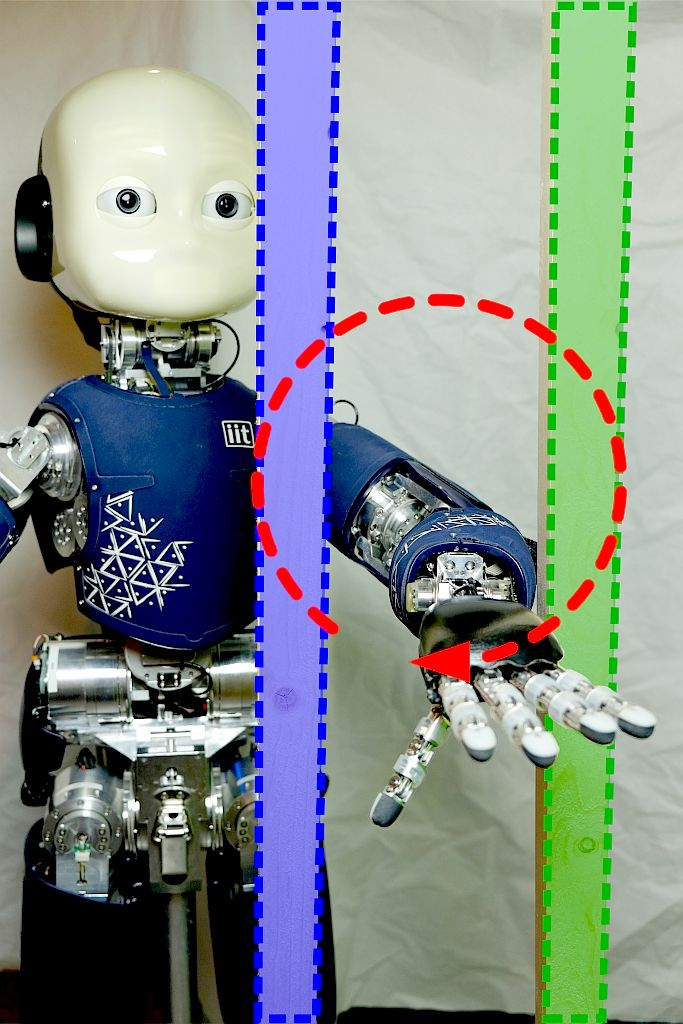
\includegraphics[width =.94\linewidth]{iCubParis02_Double_Contact}
			\caption{The robot performs a circle with its left arm. 
			The forearm collides alternatively with the left, the right or both contacts.}
			\label{fig:exp3:icuparis_experiment_bars}
		\end{minipage}	
		\hfill
		\begin{minipage}{.52\linewidth}
			\centering
			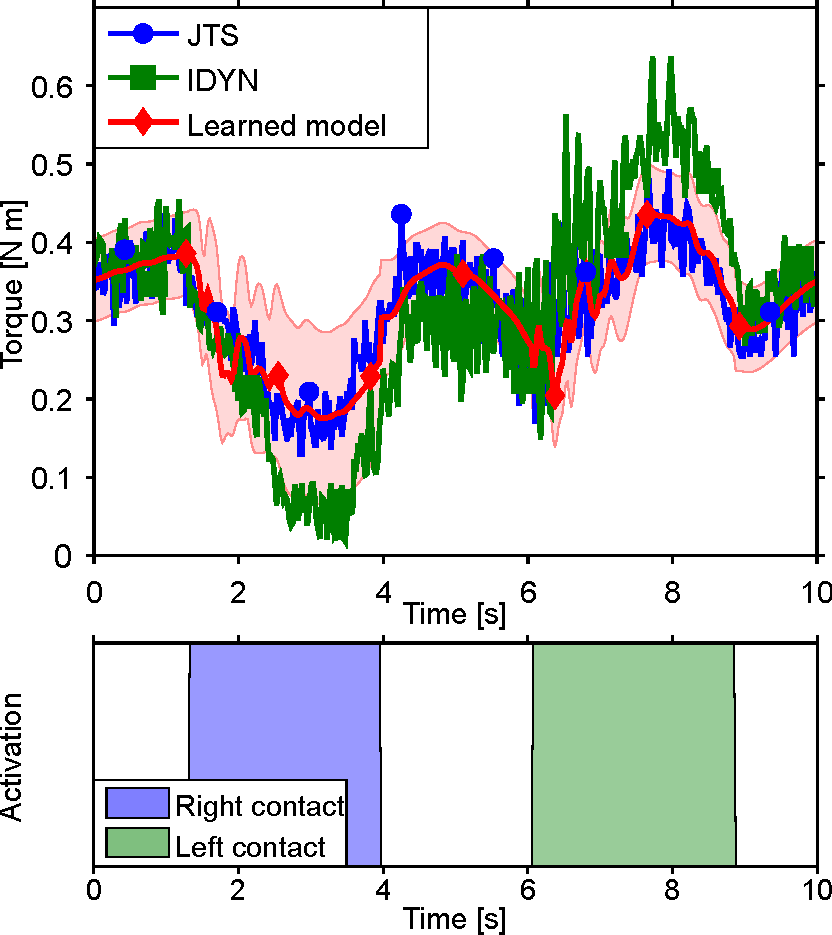
\includegraphics[width=.89\linewidth]{exp3_both}
			\caption{Prediction of torques with multiple contacts and the corresponding activation of the gating network.
			%Various models are shown, but individually, none of them correctly capture the dynamics of the system. 
			Our mixture-of-experts model combines the learned single-contact models into a multiple-contact model which outperform the analytic approach.
			}
			\label{fig:exp3:gating}
		\end{minipage}	
        %\figspace
	\end{figure}
	
INRIA, in collaboration with TUD, started to study the problem of bootstrapping the parameterized controllers proposed in T3.3. A major problem is how the controllers parameters, particularly the task weights, can be initialized or learned through trial-and-error. With the increasing abilities of humanoid robots, the number of tasks increases, together with their weights or priorities: manually specifying them through a sequence of complex manipulations becomes a major bottleneck. 
As a first step towards the offline optimization of those parameters, we evaluated the benefit of using a stochastic optimization derivative-free strategy such as \textit{Covariance Matrix Adaptation Evolution Strategy} (CMA-ES) \cite{Hansen-2001-ID362}. We report on the robustness of the optimization strategy by comparing several optimizations experiments with constant and random values for the GHC controller in Figure~\ref{fig:robust}.
The full study is detailed in the Task 4.4.

\begin{figure}[h!]
  \centering
  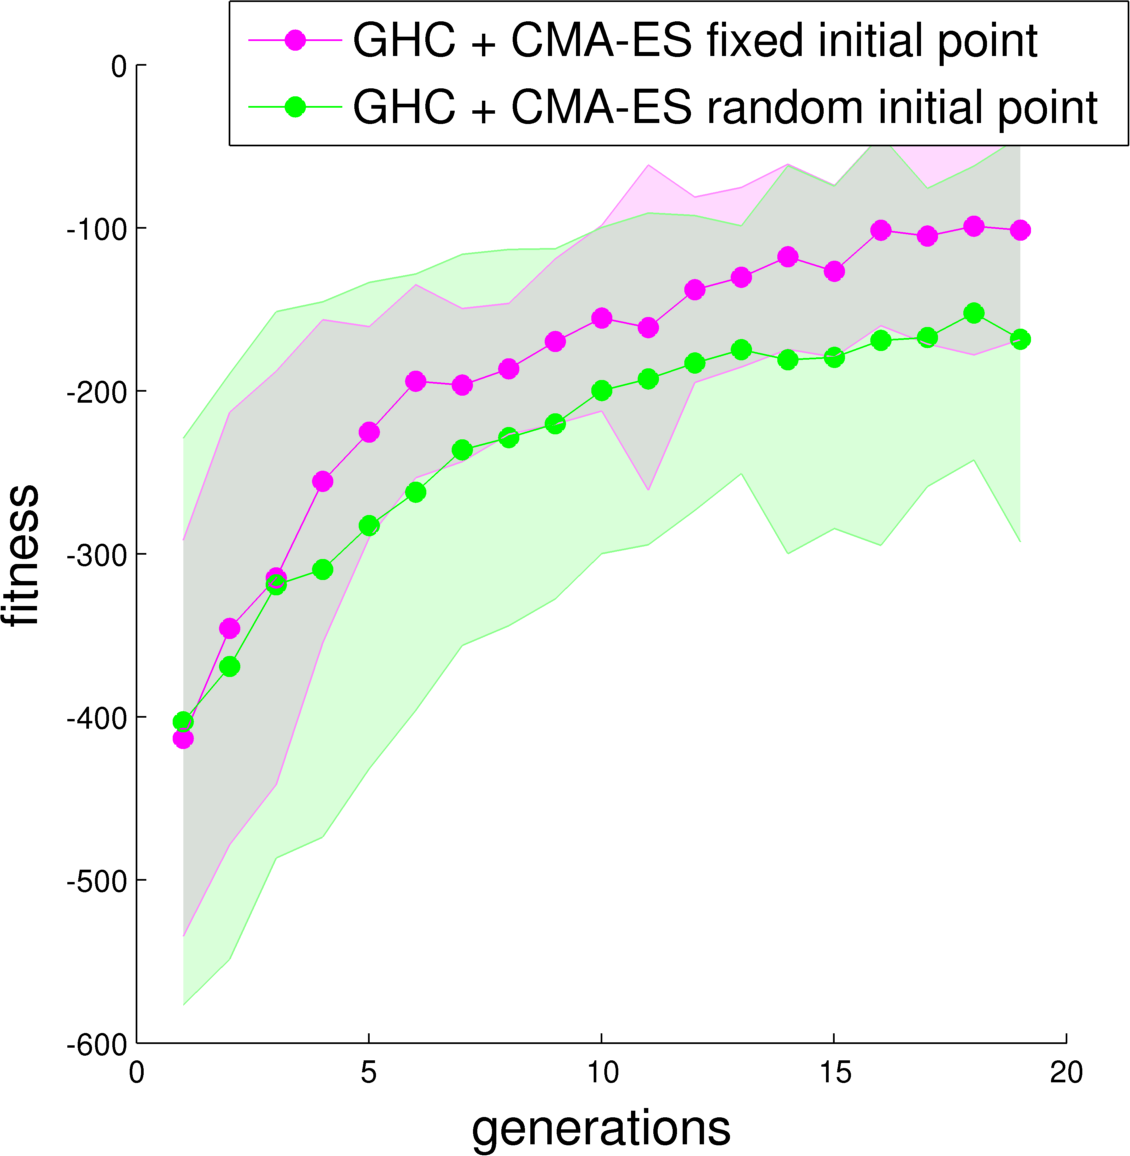
\includegraphics[width=0.5\hsize]{GHC_robust}
\caption{Learning the activation policies for GHC with CMA-ES. The policies were initialized with constant values $\alpha=0.5$ or random values between $[0,1]$. We show the mean and variance of the fitness function used for optimization for $R=20$ replicates a test experiment (see also Task 4.4).}
\label{fig:robust}
\end{figure}
